\section{ÔN TẬP CHƯƠNG 1}
\Opensolutionfile{ans}[ans/FINAL-CHAPTER1-TL]
\setcounter{ex}{0}
\begin{ex}
	Tìm số CSCN của các số sau:
	\begin{enumerate}[label=\alph*)]
		\item $78,9\pm 0,2$;
		\item $3,788\cdot10^9$;
		\item $2,46\cdot10^6$;
		\item $0,0053$.
	\end{enumerate}
	\loigiai{
		\begin{enumerate}[label=\alph*)]
			\item 3 CSCN;
			\item 4 CSCN;
			\item 3 CSCN;
			\item 2 CSCN.
		\end{enumerate}
	}
\end{ex}

\begin{ex}
	Trong quá trình thực hành tại phòng thí nghiệm, một bạn học sinh vô tình làm vỡ nhiệt kế thuỷ ngân và làm thuỷ ngân đổ ra ngoài như Hình \ref{fig:2P-2}. Em hãy giúp bạn học sinh đó đưa ra cách xử lí thuỷ ngân đổ ra ngoài đúng cách để đảm bảo an toàn.
	\begin{center}
		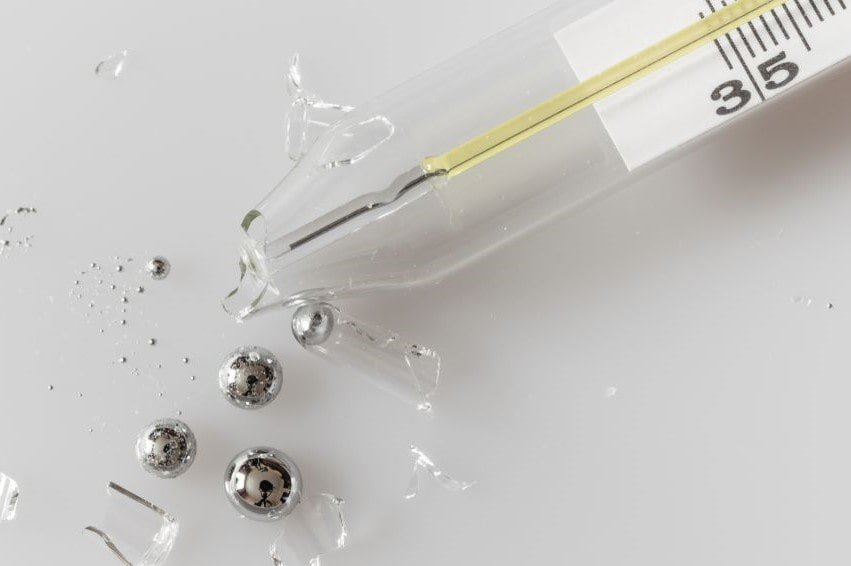
\includegraphics[width=0.3\linewidth]{figs/FINAL-CHAPTER1-2}
		\captionof{figure}{Thuỷ ngân bị đổ ra khỏi nhiệt kế}
		\label{fig:2P-2}
	\end{center}
	\loigiai{
		Cách xử lí đúng nguyên tắc an toàn: báo cho giáo viên tại phòng thí nghiệm, sơ tán các bạn học sinh ở khu vực gần đó, tắt quạt và đóng hết cửa sổ để tránh việc thuỷ ngân phát tán trong không khí. Người dọn dẹp phải sử dụng găng tay và khẩu trang để dọn sạch thuỷ ngân, tuyệt đối không được tiếp xúc với thuỷ ngân bằng tay trần.
	}
\end{ex}

\begin{ex}
	Theo em, tốc độ bay hơi của nước phụ thuộc vào những đặc điểm nào? Hãy dựa trên những hiện tượng thường thấy hằng ngày để đưa ra giả thuyết và thiết kế phương án thí nghiệm kiểm tra giải thuyết của mình.
	\loigiai{
		Nhiệt độ của nước, gió trên mặt thoáng của nước và diện tích mặt thoáng của nước.
	}
\end{ex}

\begin{ex}
	Hai người cùng đo chiều dài của cánh cửa sổ, kết quả thu được như sau:
	\begin{itemize}
		\item Người thứ nhất: $d=\xsi{120\pm1}{\centi\meter}$;
		\item Người thứ hai: $d=\xsi{120\pm 2}{\centi\meter}$;
	\end{itemize}
	Trong hai người, ai là người đo chính xác hơn? Vì sao?
	\loigiai{
		Người 1 đo chính xác hơn vì với cùng một giá trị trung bình nhưng sai số tuyệt đối trong phép đo của người 1 bé hơn sai số tuyệt đối trong phép đo của người 2.\\
		Hoặc có thể tính sai số tỉ đối $\delta_1=\SI{0.83}{\percent}$ và $\delta_2=\SI{1.67}{\percent}$. Vì $\delta_1<\delta_2$ nên người 1 đo chính xác hơn.	
	}
\end{ex}

\begin{ex}
	Một tấm bìa hình chữ nhật có chiều dài $\xsi{\left(21.3\pm0.2\right)}{\centi\meter}$ và chiều rộng $\xsi{\left(9.8\pm0.1\right)}{\centi\meter}$. Tính diện tích của tấm bìa.
	\loigiai{
		$$S=\xsi{\left(21.3\pm0.2\right)\times\left(9.8\pm0.1\right)}{\square\centi\meter}=\xsi{\left(21.3\times 9.8 \pm 21.3\times 0.1 \pm 9.8\times 0.2 \pm 0.1\times 0.2\right)}{\square\centi\meter}= \xsi{\left(209\pm4\right)}{\square\centi\meter}.$$
		Hoặc
		$$\overline{S}=\overline{d}\times \overline{r}=\xsi{21.3\times 9.8}{\square\centi\meter}=\SI{208.8}{\square\centi\meter}$$
		$$\Delta S=\left(\dfrac{\Delta d}{\overline{d}}+\dfrac{\Delta r}{\overline{r}}\right)\times \overline{S}=\SI{4.1}{\square\centi\meter}$$
		Vậy kết quả đo diện tích của tấm bìa $S=\xsi{\left(209\pm4\right)}{\square\centi\meter}.$
	}
\end{ex}

\begin{ex}
	Một học sinh đo cường độ dòng điện đi qua các đèn $\text{Đ}_1$ và $\text{Đ}_2$ như Hình \ref{fig:0001-1} được các giá trị lần lượt là 
	\begin{center}
		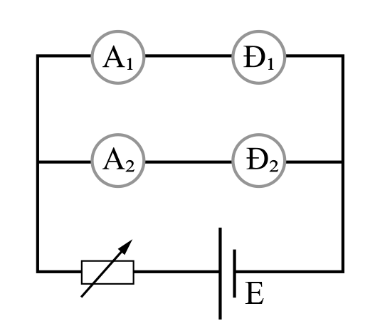
\includegraphics[width=0.3\linewidth]{figs/FINAL-CHAPTER1-1}
		\captionof{figure}{}
		\label{fig:0001-1}
	\end{center}
	$$I_1=\xsi{\left(2.0\pm0.1\right)}{\ampere}$$
	$$I_2=\xsi{\left(1.5\pm0.2\right)}{\ampere}$$
	Cường độ dòng điện mạch chính được cho bởi
	$$I=I_1+I_2$$
	Tính giá trị và viết kết quả của $I$.
	\loigiai{
		$$I=\xsi{\left(3.5\pm0.3\right)}{\ampere}.$$
	}
\end{ex}

\begin{ex}
	Một nhóm học sinh đo được hiệu điện thế giữa hai đầu một điện trở là $\xsi{\left(10.0\pm0.3\right)}{\volt}$ và cường độ dòng điện qua điện trở là $\xsi{\left(1.3\pm0.2\right)}{\ampere}$. Viết kết quả tính giá trị của điện trở.
	\loigiai{
		Ta có: $R=\dfrac{U}{I}$\\
		Giá trị trung bình $$\overline{R}=\dfrac{\overline{U}}{\overline{I}}=\SI{7.7}{\ohm}$$
		Sai số tuyệt đối:
		$$\Delta R =\left(\dfrac{\Delta U}{\overline{U}}+\dfrac{\Delta I}{\overline{I}}\right)\cdot\overline{R}=\SI{1.4}{\ohm}$$
		Vậy kết quả tính giá trị điện trở $R=\xsi{\left(7.7\pm1.4\right)}{\ohm}.$
	}
\end{ex}

\begin{ex}
	Cho bảng số liệu thể hiện kết quả đo khối lượng của một túi trái cây bằng cân đồng hồ. Em hãy xác định sai số tuyệt đối ứng với từng lần đo, sai số tuyệt đối và sai số tương đối của phép đo. Biết sai số dụng cụ là $\SI{0.1}{\kilogram}$.
	\begin{center}
		\begin{tabular}{|c|c|c|}
			\hline
			\thead{Lần đo} & \thead{$\xsi{m}{\left(\kilogram\right)}$} & \thead{$\xsi{\Delta m}{\left(\kilogram\right)}$}\\
			\hline
			1& $4,2$ & \dots\\
			\hline
			2& $4,4$ & \dots\\
			\hline
			3& $4,4$ & \dots\\
			\hline
			4& $4,2$ & \dots\\
			\hline
		\end{tabular}
	\end{center}
	\loigiai{
		\begin{center}
			\begin{tabular}{|c|c|c|}
				\hline
				\thead{Lần đo} & \thead{$\xsi{m}{\left(\kilogram\right)}$} & \thead{$\xsi{\Delta m}{\left(\kilogram\right)}$}\\
				\hline
				1& $4,2$ & $0,1$\\
				\hline
				2& $4,4$ & $0,1$\\
				\hline
				3& $4,4$ & $0,1$\\
				\hline
				4& $4,2$ & $0,1$\\
				\hline
				Trung bình &$4,3$ & $0,1$\\
				\hline
			\end{tabular}
		\end{center}
		Sai số tuyệt đối: $\Delta m=\overline{\Delta m}+\Delta m_\text{dc}=\SI{0.2}{\kilogram}$.\\
		Sai số tương đối: $\delta m=\dfrac{\Delta m}{\overline{m}}=\SI{4.65}{\percent}$.\\
		Kết quả đo: $m=\xsi{4.3\pm0.2}{\kilogram}$.
	}
\end{ex}

\begin{ex}
	Giá trị đo gia tốc rơi tự do $g$ có thể được xác định bằng cách đo chu kì dao động của con lắc đơn có chiều dài $\ell$. Mối quan hệ giữa $g, T$ và $\ell$ là 
	$$g=4\pi^2\left(\dfrac{\ell}{T^2}\right)$$
	Trong một thí nghiệm, đo được:
	$$\ell=\xsi{\left(0.55\pm0.02\right)}{\meter}; T=\xsi{\left(1.50\pm0.02\right)}{\second}$$
	Tìm giá trị và viết kết quả của $g$.
	\loigiai{
		Giá trị trung bình:
		$$\overline{g}=4\pi^2\cdot\dfrac{\overline{\ell}}{\overline{T}^2}$$
		Sai số tuyệt đối
		$$\Delta g=\left(\dfrac{\Delta \ell}{\overline{\ell}}+2\cdot\dfrac{\Delta T}{\overline{T}}\right)\cdot\overline{g}=\SI{0.6}{\meter\per\square\second}$$
		Kết quả đo:
		$$g=\xsi{\left(9.7\pm0.6\right)}{\meter\per\square\second}.$$
	}
\end{ex}

\begin{ex}
	Một học sinh dùng thước có ĐCNN là $\SI{1}{\milli\meter}$ và một đồng hồ đo thời gian có ĐCNN $\SI{0.01}{\second}$ để đo 5 lần thời gian chuyển động của một chiếc xe đồ chơi chạy bằng pin từ điểm $A$ đến điểm $B$. Kết quả đo được cho ở bảng sau
	\begin{center}
		\begin{tabular}{|c|c|c|c|c|}
			\hline
			\thead{Lần đo}& \thead{$\xsi{s}{\left(\meter\right)}$} &\thead{$\xsi{\Delta s}{\left(\meter\right)}$} & \thead{$\xsi{t}{\left(\second\right)}$} & \thead{$\xsi{\Delta t}{\left(\second\right)}$}\\
			\hline
			1 & $0,546$ & \dots & $2,47$ & \dots\\
			\hline
			2 & $0,554$ & \dots & $2,51$ & \dots\\
			\hline
			3 & $0,549$ & \dots & $2,42$ & \dots\\
			\hline
			4 & $0,560$ & \dots & $2,52$ & \dots\\
			\hline
			5 & $0,551$ & \dots & $2,48$ & \dots\\
			\hline
		\end{tabular}
	\end{center}
	\begin{enumerate}[label=\alph*)]
		\item Nêu nguyên nhân gây ra sự sai khác giữa các lần đo?
		\item Tính sai số tuyệt đối và sai số tỉ đối của phép đo $s$, $t$.
		\item Biểu diễn kết quả đo $s$ và $t$.
		\item Tính sai sối tỉ đối $\delta v$ sai số tuyệt đối $\Delta v$. Biểu diễn kết quả tính $v$.
	\end{enumerate}
	\loigiai{
		\begin{enumerate}[label=\alph*)]
			\item Nguyên nhân gây ra sai khác giữa các lần đo: Do cấu tạo của dụng cụ thí nghiệm, thao tác khi đo chưa chuẩn xác.
			\item $\Delta s=\SI{0.0055}{\meter}$; $\Delta t=\SI{0.035}{\second}$.
			\item $s=\xsi{0.5520\pm0.0055}{\meter}$; $t=\xsi{2.480\pm0.035}{\second}$.
			\item $\delta v=\SI{2.41}{\percent}$; $\Delta v=\SI{0.0054}{\meter\per\second}$.\\
			Kết quả tính: $v=\xsi{0.2226\pm0.0054}{\meter\per\second}$.
		\end{enumerate}
	}
\end{ex}
\Closesolutionfile{ans}